%\renewcommand{\chapterheadstartvskip}{\vspace*{0 cm}}

\chapter{Theoretische Grundlagen}
\label{chap:theoretischegrundlagen}


\section{Model Predictive Control}
\label{chap:mpc}


\acrlong{mpc} an sich ist eine Methodik zur Steuerung von Systemen. Diese versucht zunächst, zu sich periodisch wiederholenden, diskreten Zeitpunkten das Verhalten eines Systems in der Zukunft -- also einer immer gleich weit in die Zukunft hineinreichenden Periode -- zu beschreiben. Hierzu bedient \acrlong{mpc} sich der Kenntnis des aktuellen Zustandes und eines physikalischen-mathematischen Modells des Systems, um dessen zukünftiges Verhalten \Gun vorherzusagen \Gob bzw. abzubilden. Des Weiteren wird versucht das Verhalten des Systems mit minimalem Aufwand zu beeinflussen, um einem eigens- oder vordefinierten Zielkriterium zu folgen \acrlong{bzw} diesem zu entsprechen.




\section{Technische Grundlagen zur Kommunikation mit Bussystemen}
\label{sec:grundlagenbus}
In diesem Kapitel werden die Grundlagen von Hard- und Software beleuchtet die für die Kommunikation der Steuerung mit den einzelnen Anlagenteilen benötigt werden.
Diese umfassen zunächst Bussysteme im Allgemeinen und werden anhand des spezifischen/konkreten Anwendungsfalls Modbus erläutert.
Die Einführung wird sich an die Strukutr nach \cite{schn06} anlehnen.

\subsection{OSI-Kommunikationsmodell}
Hier wird das OSI mit Schichten--> Referenzieren von Schichten in den Folgenden.
Aufgrund der großen Anzahl verschiedener technischer Systemen existieren auch viele verschiedene Arten der Kommunikation von technischen Systemen. Bei einer genaueren Betrachtung dieser Kommunikation wird ersichtlich, das diese oftmals ähnlich abläuft und sich durch ein Meta-Schema beschreiben lässt \cite[S.~8]{schn06}. Um die Kommunikation auch über diese verschiedenen Systeme hinweg zu ermöglichen und zu formalisieren, wurde von der \textit{International Organization for Standardization} 1984 ein abstraktes Referenz-Modell entwickelt, dass in der \textit{ISO 7498-1} beschrieben ist und zur Entwicklung und Verbesserung von Standards der des Informationsaustauschs und als Referenz für die Konsistenz aller bestehenden Standards  dient \cite[S.~1]{osi96}. Das Ziel des Modells (design intend) war/ist es, eine Menge von Standards zu schaffen damit es autonomen Systemen möglich ist miteinander zu kommunizieren \cite[S.~4]{osi96}.

Das sogenannte \acrlong{osi} (\acrshort{osi}) wird zunächst allgemein erläutert, da die Kommunikation von technischen Systemen im Rahmen dieser Arbeit eine zentrale Rolle spielt, und wird anschließend im Kontext mit den eingesetzten Protokollen/Schnittstellen der verschiedenen eingesetzten Technologien angewendet.

Zunächst wird im Standard definiert womit sich das Modell beschäftigt und abgegrenzt was im Modell berücksichtigt wird und was nicht \cite[S.~3]{osi96}:

\begin{quote}
\textit{\Gun OSI is concerned with the exchange of information between open systems (and not the internal functioning of each individual real open system).\Gob}
\end{quote}

Das \acrshort{osi} beschäftigt sich also zentral mit dem Austausch von Informationen und allen dazugehörigen Aufgaben. Diese sind sehr umfangreich und umfassen folgende Aufgabenbereiche/bzw werden jeweils/nur bezogen auf den Austausch von Informationen und wie folgt beschrieben, \cite[S.~3f.]{osi96}:.

\begin{itemize}
\item die physischen Medien zur Vernetzung von offenen Systemen,
\item die Vernetzung (an sich) von offenen Systemen,
\item die Übertragung von Daten, umfassenderweise eine Kooperation von Systemen
\end{itemize}

Bezogen auf den Austausch von Daten überschneiden sich die physischen Medien mit der Vernetzung und meinen also die Infrastruktur und deren Architektur, die zur Übertragung zur Verfügung steht. Bei der Kooperation von Systemen zur Datenübertragung sind weitaus mehr Aspekte zu beachten: Zunächst die Synchronisation der Prozesse, die Daten austauschen wollen. Des Weiteren die Darstellung der auszutauschenden Daten und deren eventuell notwendigen Transformation um mit einem anderen System kompatibel zu sein. Weitere wichtige Aufgaben sind die Datenspeicherung sowie deren Integrität und die Sicherheit des Austausch hinsichtlich Fehler und Einsicht von Außen \cite[S.~4]{osi96}.

Wie leicht zu erkennen ist, ist die Kommunikation zwischen verschiedenen technischen Systemen sehr umfangreich/komplex/kompliziert. Daher wird der Kommunikationsprozess im \acrshort{osi} stark abstrahiert und zunächst in 7 verschiedene, abstrakte Ebenen aufgeteil um die einzelnen Aufgabenbereiche des Kommunikationsprozesses anfallen in Teilaufgaben zu gliedern bzw. zusammenzufassen, wie in Abbildung \ref{fig:osi} dargestellt.

\begin{figure}
\centering
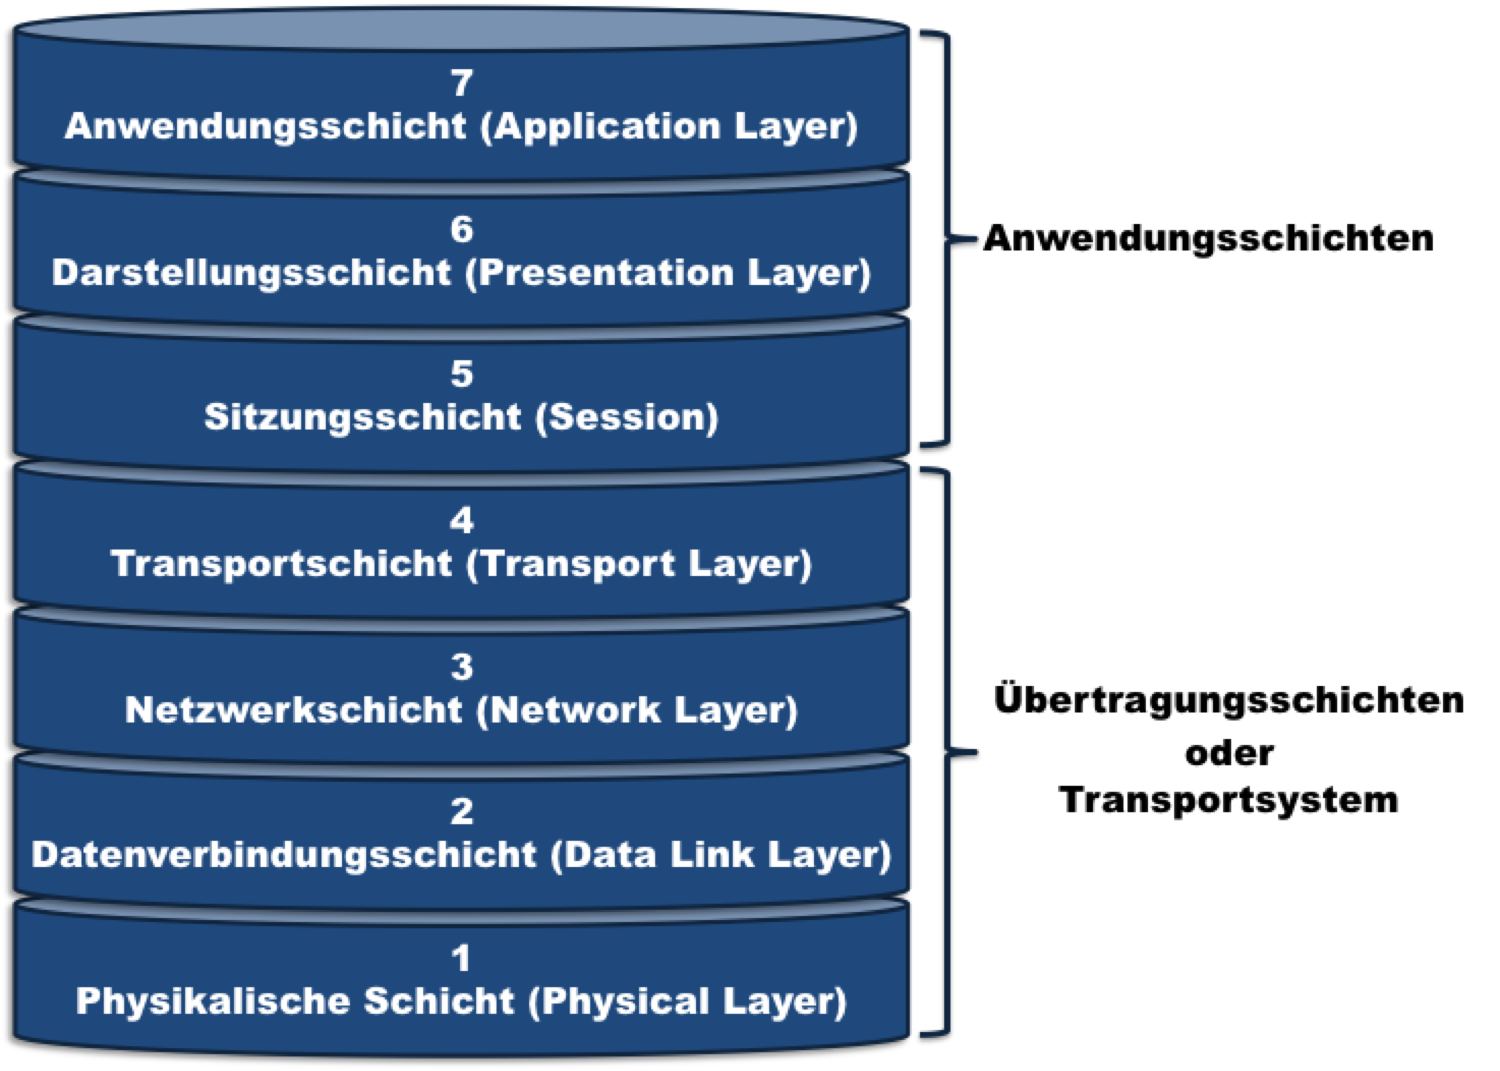
\includegraphics[width=0.8\textwidth]{abbildungen/20160112_osi}
\caption[Die sieben Schichten des Open System Interconnection Modells]{Die sieben Schichten des \textit{Open System Interconnection} Modells verändert nach \cite[S.~10]{schn06} und \cite[S.~28]{osi96}}
\label{fig:osi}
\end{figure}

Jede Ebene hat dann klar definierte Teilaufgaben, die der Kommunikation dienen. Diese Ebenen werden Schichten genannt und haben klar definierte Schnittstellen/interfaces zu ihren Nachbarschichten. An diesen Schnittstellen stellen die einzelnen Schichten Dienste bereit die von den anderen Ebenen genutzt werden können. Durch diesen Aufbau können Schichten einfach bearbeitet oder ausgetauscht werden, ohne die Gesamtfunktionalität zu gefährden. Dadurch kann ein System auch aus Komponenten verschiedener Hersteller zusammengesetzt werden, diese Architektur dient also als Basis für offene Systeme. Wie in Abbildung \ref{fig:osi} ebenfalls dargestellt ist, werden die Schichten eins bis vier auch als Übertragungsschichten oder Transportsystem zusammengefasst und sind für die Datenübertragung zwischen den Systemen verantwortlich. Die Schichten fünf bis sieben werden gemeinsam als Anwendungsschichten bezeichnet und stellen die Zusammenarbeit bei der Datenübertragung zwischen der Anwendersoftware und dem Betriebssystem sicher \cite[S.~8f.]{schn06}.

Im Folgenden wird kurz auf die einzelnen Schichten eingegangen bevor das Zusammenwirken der einzelnen Schichten anhand eines Beispiels verdeutlicht wird.

Die Schicht eins -- die physikalische Schicht -- Möglichkeiten zur Verfügung und die phsysikalische Datenübertragung der einzelnen Bits \cite[S.~49f.]{osi96}. Sie legt also die mechanischen, wie zb. stecker(endsystemkopplung), zurodnung der pins und kabelspezifikationen, elektrischen, art der codierung Spannungspegel etc., fest, idr Standards wie RS/EIA 232, RS/EIA 422, RS/EIA 485, oder aber auch Glasfaserstrecke. Wichtig ist dabei, dass diese lediglich die tatsächlcihe Strecke spezifiziert und nicht das physikalische Medium selbst ist und die Kommunikation unabhängig von der konkreten Ausprägung der Schicht ist \cite[S.~9]{schn06}.

Die zweite Schicht -- die Datenverbindungsschicht -- ist für verschiedene Verbindungsmodi 



\subsection{Bussysteme} 
Um ganz allgemein Prozesse überwachen und steuern zu können müssen unter den einzelnen Einheiten innerhalb eines Systems Informationen ausgetauscht werden. Dazu werden Kommunikationssysteme benötigt mit Hilfe derer Kommunikation erfolgen kann. Diesem Zweck dienen Bussysteme
Info/Quelle 
%%W. Kriesel, T. Heimbold, D. Telschow: Bustechnologien für die Automation, Hüthig GmbH, Heidelberg 1998
Bussysteme lassen sich anhand verschiedener Kriterien einteilen bzw klassifizieren. Im Rahmen dieser Arbeit wird der Modbus eingesetzt weshalb im Folgenden die Kriterien zunächst sehr allgemein zum Verständnis des Krieteriums beschrieben werden. Die verschiedenen Ausprägungen der einzelnen Kriterien werden lediglich die für Modbus relevanten detailliert beschrieben.

\subsubsection{Netzwerk und Topologie}
Verknüpft man einzelne Prozesseinheiten -- im folgenden Teilnehmer des Netzwerks -- miteinander über Verbindungsleitungen, über die Informationen übertragen werden können, entstehen dabei Netzwerke. Diese Netzwerke können unterschiedlich ausgeprägt sein und werden anhand ihrer geometrischen Anordnung, der Netzwerktopologie, unterschieden.
--> Teilnehmer im Netzwerk definieren

Die einfachste Art zwei Teilnehmer miteinander zu verbinden ist eine direkte Zweipunktverbindung mit einer Leitung. Jedoch würde mit jeder steigenden Zahl von Teinehmern auch überproportional mehr Verbindungsleitungen benötigt um alle Teilnehmer miteinander zu verbinden. Dies hätte für große Zweipunbktverbindungsnetzwerke. die auch als vermaschtes Netz bezeichnet werden, eine unübersichtliche große Anzahl von Schnittstellen, einen extrem hohen Verkabelungsaufwand und damit verbundene hohe Kosten zur Folge. Um dies zu vermeiden ergeben sich noch verschiedene andere Möglichkeiten zur Anordnung von Teilnehmern in Netzwerken \cite[S.~1f.]{schn06}.

Die Zweipunktverbindungen sind wie oben beschrieben mit einem hohen Verkabelungsaufwand verbunden, weshalb bei großen Netzwerken oftmals zu einer Linienstruktur übergegangen wird. Diese wird auch Linienstruktur genannt und wird auch von der Modbus-Technologie empfohlen/vorgeschrieben. Charakteristisch dafür ist, dass alle Teilnehmer eine gemeinsame Verbindungsleitung zur Kommunikation nutzen. Dazu gibt es ein sogenanntes, langes Buskabel entlang dessen die einzelnen Teilnehmer mit Hilfe von kurzen Stichleitungen angebunden sind, wie auf Abbildung \ref{fig:bus_struktur} zu sehen ist.

\begin{figure}
\centering
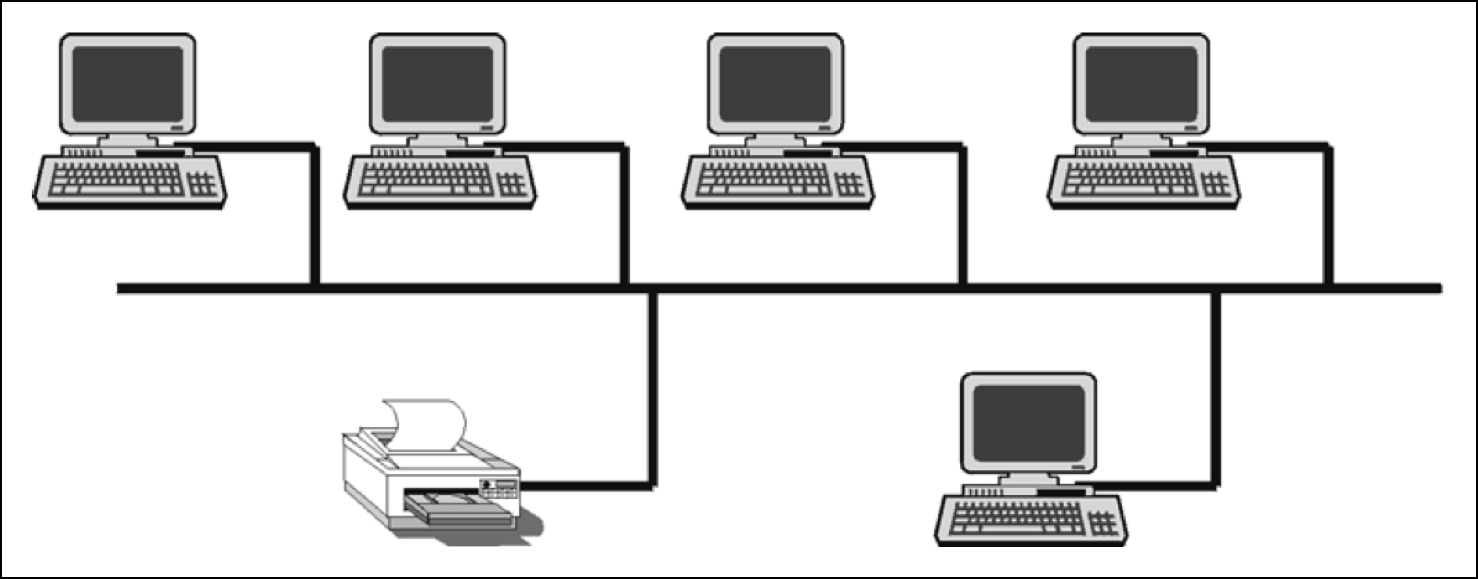
\includegraphics[width=\textwidth]{abbildungen/20160109_busstruktur}
\caption[Linienstruktur]{Linienstruktur aus \cite[S.~3]{schn06}}
\label{fig:bus_struktur}
\end{figure}

Dadurch wird der Verkabelungsaufwand auch für sehr große Netzwerke stark reduziert und auch die Anzahl an Schnittstellen der Teilnehmer auf eine einzige reduziert. Jedoch wird dadurch das gleichzeitige Senden von Teilnehmern erschwert und es müssen sogenannte Buszugriffsverfahren definiert werden, die nichts weiter als Regeln sind die den Zugriff auf den Bus festlegen. Da die Kommunikation auf einer einzigen Leitung stattfindet und ständig alle Teilnehmer alle Sendungen verfolgen wird der Sender durch diese Parallelschaltung der Empfänger stark belastet. Da die Bus-Längen meist sehr lang sind ( hunderte Meter) ist die Leitungslänge im Bezug auf die zu übertragende Wellenlänge nicht mehr vernachlässigbar. Deshalb müssen beide Enden der Busleitung mit Leitungsabschlusswiderständen versehen werden sowie die Leitungslänge und die Teilnehmer je Netzwerk begrenzt werden. Der Leistungs- und Kapazitätswiderstand einer Leitung sind von der Länge der Leitung abhängig und werden durch das Ersatzschaltbild eines RC-Gliedes repräsentiert, wie in Abbildung \ref{fig:bus_impuls}a zu sehen ist. Durch diese Widerstände wird eine Impulsverzerrung $\delta t$ auf der Leitung ausgelöst, die somit mittelbar auch von der Leitungslänge abhängt. Je länger die Leitung desto größer die beiden Widerstande und desto größer ist die Impulsverzerrung $\delta t$, da der Kondensator C\_{Leitung} mehr Zeit zum Aufladen benötigt und die Lastspannung sinkt, wie in Abbildung \ref{fig:bus_impuls}b und \ref{fig:bus_impuls}c dargestellt. Dadurch wird die maximale Frequenz der Datenübertragung beschränkt (auf den Kehrwert der Impulsverzerrung f=1/t). Dies bedeutet das die Frequenz der Datenübertragung entlang der Leitung von ihrer Länge mittelbar abhängig ist, da ansonsten der Empfänger den Wechsel des logischen Zustand nicht mehr registrieren kann \cite[S.~3ff.]{schn06}.

\begin{figure}
\centering
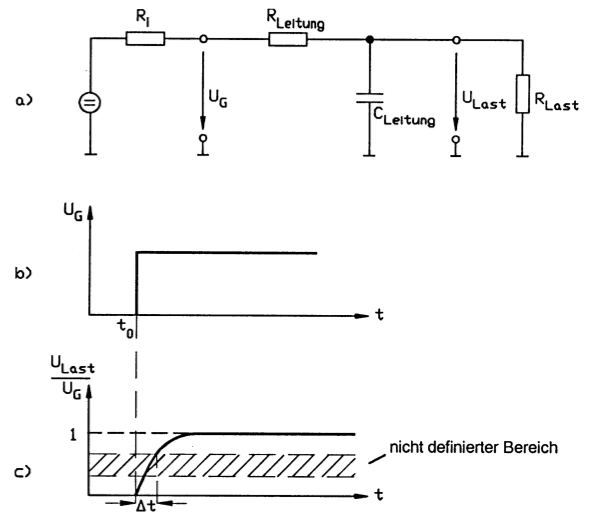
\includegraphics[width=0.6\textwidth]{abbildungen/20160110_impulsbus}
\caption[Impulsverzerrung auf einer Leitung]{Impulsverzerrung auf einer Leitung: a) Ersatzschaltbild der Anordnung b) Ausgangsspannung des Generators c) Empfängerspannung aus \cite[S.~4]{schn06}}
\label{fig:bus_impuls}
\end{figure}

Weitere Bus-Strukturen sind die Baumstruktur, die eine Weiterentwicklung der Linienstruktur ist und auf Abbildung \ref{fig:baum_struktur}. Dabei werden einzelne Linienstrukturen durch Verstärkerelemente, sogenannte  Repeater, miteinander verbunden und es können dadurch größere Flächen als mit der Linienstruktur vernetzt werden. \cite[S.5~f.]{schn06}.
--> Galvanische Trennung und Abschirmung 
Diese Struktur ist insofern interessant, da es also im Rahmen dieser Arbeit Anlage noch eine nachträgliche Erweiterung/Vergrößerung der geplanten Anlage ermöglicht.

Modbus was da oben steht, Teilnehmer kabellängen etc.

\begin{figure}
\centering
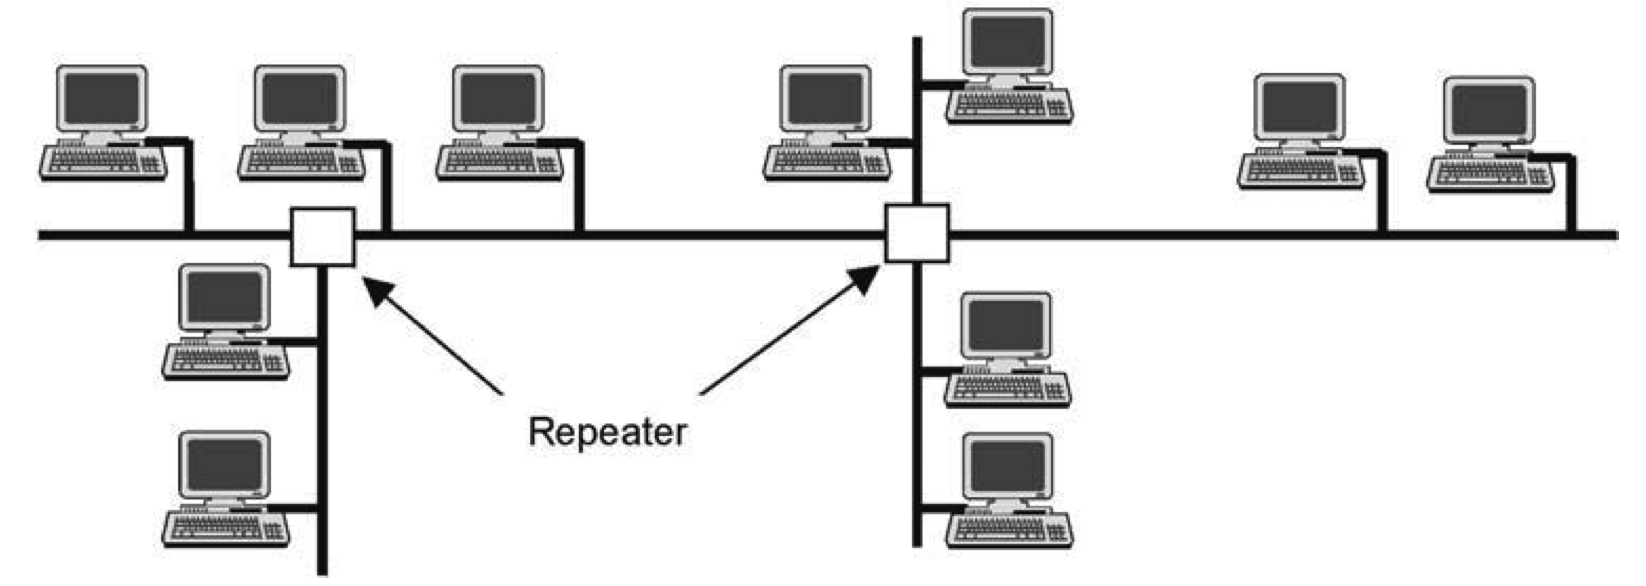
\includegraphics[width=\textwidth]{abbildungen/20160110_baumstruktur}
\caption[Baumstruktur]{Baumstruktur aus \cite[S.~5]{schn06}}
\label{fig:baum_struktur}
\end{figure}

Weitere wichtige Netzwerk Topologien, die für das Verständnis dieser Arbeit keine weitere Relevanz haben, jedoch genannt werden sollten sind die Ring- und die Stern-Struktur. Die Ring-Struktur ist dadurch gekennzeichnet, ein physikalischer Ring mit Zweipunktverbindungen aufgebaut wird in dem über Teilnehmer hinweg kommuniziert wird. Die Stern-Topologie ist durch eine Zentralstation gekennzeichnet, die mit allen Teilnehmer verbunden ist und über die die gesamte Kommunikation abläuft \cite[S.~6f.]{schn06}.

\subsubsection{Elektrisches EIA-485 Netzwerk/Interface}
Hier wird EIA / RS485 dargestellt und abgegrenzt zu RS 232 und RS 422

\subsubsection{Hardware}
Kabel, Belegung

\subsection{Modbus}
Hier wird das Modbusprotokoll nach \cite{mod12} und \cite{mod06ser} und \cite{mod06tcp}  
Und nach hier wird das Modbusprotokoll nach \cite[S.5]{mod12} und \cite[S.5]{mod06ser} und \cite[S.5]{mod06tcp}









\section{Technische Grundlagen zur Modellbildung}
\label{sec:grundlagenmodell}
In diesem Kapitel werden die technischen Grundlagen zur Bildung eines mathematischen Modells des Raumes erläutert.
Themrodym systeme
1. HS thermo
Wärmeübertragung

\subsection{Thermodynamische Systeme}
Im Raummodell müssen Energieströme, genauer betrachtet Wärmeströme, untersucht werden. Um dieses thermodynamischen Vorgänge mit Hilfe von Bilanzierungsgleichungen zu beschreiben, folgt zunächst ein kurze Einführung in die Thermodynamische Systembildung nach \cite[S.~11ff.]{ba12}.

\textit{Thermodynamische Systeme} werden durch den zu untersuchenden Raum abgegrenzt. Sie dienen dem Zweck der Bilanzierung von Massen- und Energieströmen und alles was diesen abgegrenzten Raum an den Systemgrenzen umgibt wird als Umgebung bezeichnet. Die begrenzenden Flächen können gedanklicher, physischer oder beider Natur zugleich sein, wichtig ist jedoch das die Systemgrenzen eindeutig festgelegt sind \cite[S.~11]{ba12}.

Anhand der Eigenschaften von den Systemgrenzen lassen sich die thermodynamischen Systeme weiter differenzieren.
Solche Systeme, deren Grenzen undurchlässig für Materie sind, werden als \textit{geschlossene Systeme} bezeichnet und werden durch eine konstante Stoffmenge innerhalb des Systems gekennzeichnet. Die Grenzen eines geschlossenen Systems sind meistens räumlich anhand eines fixen Volumens definiert, können aber auch beweglich sein, wie z.B. das Volumen einer vorgegebenen Stoffmenge unabhängig von dessen räumlicher Ausdehnung \cite[S.~12]{ba12}.

Sind die Grenzen von thermodynamischen Systemen für Materie durchlässig, werden diese als \textit{offene Systeme} bezeichnet. In der Regel werden diese von Stoffströmen durchflossen und durch räumlich festgelegte Grenzen beschrieben. Diese werden in der Literatur auch als \textit{Kontrollraum} oder \textit{Kontrollvolumen} bezeichnet \cite[S.~12]{ba12}.

Ein \textit{abgeschlossenes System} umfasst in der Regel mehrere Systeme oder ein einzelnes System und dessen Umgebung, so dass es zwischen den Grenzen des abgeschlossenen Systems und seiner Umgebung keine Wechselwirkungen gibt. Die Systemgrenzen werden also so gelegt, dass über sie hinweg keine \acrlong{bzw} keine relevanten\footnote{\textit{Relevant} im Sinne von kaum messbarer Fluss und nicht messbare Auswirkung auf das System.} Flüsse von Materie und Energie \cite[S.~13]{ba12}.

Nach der Abgrenzung folgt die \textit{Beschreibung} von thermodynamischen Systemen und dessen \textit{Eigenschaften}. Diese erfolgt durch \textit{Variablen} und \textit{physikalische Größen} die ein System kennzeichnen. Falls die Variablen feste Werte annehmen werden diese als \textit{Zustandsgrößen} bezeichnet, da sie den \textit{Zustand} eines Systems bestimmen \cite[S.~13]{ba12}. Im Rahmen der Modellbildung in Kapitel \ref{chap:modellbildung} ist es ausreichend die Vorgänge und Effekte auf systemischer Ebene zu betrachten, wodurch sich Modelle mit wenigen Variablen und physikalischen Größen beschreiben lassen.

Die Variablen lassen sich in \textit{äußere Größen}, welche den mechanischen Zustand eines Systems beschreiben\footnote{Zum Beispiel die Koordinaten im Raum oder die relative Geschwindigkeit zum Beobachter)}, und \textit{innere Größen} gliedern, welche den thermodynamischen Zustand, also die Eigenschaften der Materie innerhalb der Systemgrenzen, beschreiben\cite[S.13~f.]{ba12}.

Innerhalb der Grenzen eines thermodynamischen Systems, und damit implizit auch für das Raummodell\footnote{Diese Annahme wird im Kapitel \ref{chap:schlussteil} noch überprüft und kritisch hinterfragt werden müssen} wird \textit{Homogenität} angenommen. Dies bedeutet, dass die physikalischen Eigenschaften, wie \acrlong{zb} Temperatur und Druck, sowie die chemische Zusammensetzung an jeder Stelle innerhalb des Systems homogen ist, also die gleiche Ausprägung besitzt \cite[S.15]{ba12}.

Da wir im Rahmen der Modellbildung Zustände betrachten müssen auch deren Änderungen genauer untersucht werden. Die \textit{Zustandsänderungen} eines Systems werden durch Änderungen von Energie oder Materie über dessen Grenzen hinweg bedingt und finden meist im Austausch der Umgebung statt. Während einer solchen Änderung des Systemzustands wird ein Prozess durchlaufen, der eine zeitliche Abfolge von Ereignissen ist. Eine Änderung des Zustands eines Systems mit der gleichen Wirkung kann also durch verschiedene Prozesse bewirkt werden. Daher beschreibt ein \textit{Prozess} nicht nur die Veränderung des Zustands sondern viel mehr die Beziehungen zwischen einem System und seiner Umgebung \cite[S.21~f.]{ba12}.

Ein Prozess kann aber auch innerhalb eines Systems stattfinden, dass heißt ohne äußere Einwirkungen. Dies geschieht zum durch das Aufheben innerer Hemmungen oder dem Wegfall Zwängen von Außen. Diese Prozesse laufen in abgeschlossenen Systemen meist von selbst ab und streben als Ziel einen ausgeglichenen, also homogenen, Endzustand an. \textit{Ausgleichsprozesse} dienen somit dazu, einen \textit{Gleichgewichtszustand} zu erreichen und repräsentieren Wechselwirkungen zwischen verschiedenen Teilen eines abgeschlossenen Systems. Dabei gleichen sich die Zustandsgrößen von einzelnen Subsystemen wie zum Beispiel der Druck oder die Temperatur einander an. Der Gleichgewichtszustand wird also durch die Zustände in den einzelnen Subsystemen bestimmt und ist dadurch charakterisiert, dass ein System diesen Zustand nicht von sich aus sondern nur durch äußere Eingriffe verlässt, zum Beispiel durch eine Veränderungen in der Umgebung. Die Erfahrung lehrt, dass ein System einem Gleichgewichtszustand entgegen strebt, wenn es sich selbst überlassen wird \cite[S.22~f.]{ba12}.
Im Rahmen der Modellbildung in Kapitel \ref{chap:modellbildung} nehmen diese \textit{Ausgleichsprozesse} eine zentrale Rolle ein, weil der Großteil an Änderungen von einzelnen Zustandsgrößen innerhalb des Raumes darauf zurückgeführt werden können. 

\subsection{Erster Hauptsatz der Thermodynamik}
Der erste Hauptsatz der Thermodynamik wird im Folgenden als allgemeiner Energieerhaltungssatz formuliert und anschließend angewendet um eine Energiebilanzgleichung für geschlossene thermodynamische Systeme zu erhalten.

Der erste Hauptsatz der Thermodynamik erweitert den mechanischen Energieerhaltungssatz um die Energieformen Wärme und innere Energie. Er handelt ganz allgemein vom Prinzip der Energieerhaltung und  dient er der Bilanzierung von Systemen \cite[S.~43]{ba12}.

Die Gesamtenergie eines Systems \textit{\gls{e}} setzt sich zusammen aus der potenziellen \textit{\gls{epot}} und kinetischen Energie \textit{\gls{ekin}} wie in der Mechanik und wird durch die innere Energie \textit{ \gls{u}} ergänzt \cite[S.~49]{ba12}:

\begin{equation}
\label{eq:energie}
E := E_{pot} + E_{kin} + U
\end{equation}

Im weiteren Verlauf der Arbeit werden nur ortsfeste Systeme betrachtet die sich dadurch auszeichnen, dass deren potenzielle Energie  \gls{epot} in etwa konstant ist. Weiterhin erfahren sie im betrachteten Intertialsystem Erde auch nur sehr kleine Änderungen in ihrer Geschwindigkeit, weshalb auch die kinetische Energie \gls{ekin} in etwa konstant ist.  Da die Änderungen der mechanischen Energien in Bezug auf die Änderung der inneren Energie sehr klein sind werden im Folgenden nicht weiter betrachtet und die Gesamtenergie eines Systems \gls{e} vereinfacht und lediglich aus der inneren Energie bestehend angenommen.

Die innere Energie hängt von der spezifischen Wärmekapazität \gls{cp}, der Masse eines Systems \gls{msys} und der Temperatur \gls{t} \acrlong{bzw} \gls{T} ab \cite[S.~54]{ba12}:

\begin{equation}
\label{eq:innereenergie}
U := m*c_p*T=m*c_p*t+u_0,~mit~t=T-T_0
\end{equation}

Nach dem Prinzip der Energieerhaltung, kann die Energie eines Systems also weder erzeugt noch vernichtet werden sondern lediglich durch den Energietransport über dessen Grenzen hinweg verändert werden. Daraus ergeben sich folgende qualitative Formen des Energietransports \cite[S.~48f.]{ba12}:

\begin{itemize}
	\item Die Arbeit \gls{w}, die entweder von oder an einem System verrichtet wird, in differentieller Form die Leistung \gls{p}.
	\item Die Wärme \gls{q}, die entweder in das System hinein- oder herausfließt, in differentieller Form der Wärmestrom \gls{qdot}.
	\item Der Transport von Materie, also das Einbringen oder Wegnehmen von Masse \gls{m} eines System, in differentieller Form die Materialflüsse \gls{mdot}.
\end{itemize}

Mit der zuvor getroffenen Annahme, dass die innere Energie der des Systems entspricht, und unter Beachtung der Vorzeichenkonvention, welche besagt dass zugeführte Energie positiv und abgeführte Energie negativ zu bewerten ist, lassen sich die Änderungen der Energie eines Systems mit der folgenden Gleichung quantitativ beschreiben \cite[S.~54]{ba12}:

\begin{equation}
\label{eq:hauptsatz}
\begin{split}
\Delta U & = Q + W + m_{in}*c_{p}*T_{in}-m_{out}*c_{p}*T_{out} \\ ~& \mathrm{beziehungsweise~in~differentieller~Form}\\
\frac{dU}{dt}=\dot{U} & =\dot{Q}+P+\dot{m}_{in}*c_{p}*T_{in}-\dot{m}_{out}*c_{p}*T_{out}
\end{split}
\end{equation}


\subsection{Wärmeübertragung}
% Here we go

Da zur Betsimmung und Steuerung einer Raumheizungsnalage die Betrachtung von Wärmeströmen unumgänglich ist werden die Grundlagen dazu im Folgenden erläutert.
Die Wärmeübertragung kann grundsätzlich nur durch zwei Arten stattfinden, durch Strahlung, die ohne stofflichen Träger durch elektromagnetische Wellen erfolgt, welche keine weitere Relevanz für weitere Betrachtungen hat und deshalb hier nicht erläutert wird, und durch die Wärmeleitung, die sich wiederum in die Leitung und die Konvektion aufteilt. \cite[S.~3f.]{bo14}

Die Wärmeübertragung wird druch den Wärmestrom $\dot{Q}$ beschrieben, der quantifiziert wieviel Wärme pro Zeiteinheit $[W]$ übertragen wird \cite[S.~5]{bo14}.
Für die weitere Betrachtung im Rahmen dieser Arbeit ist lediglich die Wärmeleitung ohne KOnvektion von Relevanz, weshalb diese nun näher erläutert wird.
Kinetische Kopplungsgleichung\cite[S.~7]{bo14}
Gleichung Qdot =k*A*deltaT
Geben Wärmestrom als Funktion an von verschiedenen Paramatern, hier Fläche an der Austausch stattfindet, Temperaturdifferenz und Wärmedurchgangszahl bzw Wärmeübergangszahl an.
Wärmedurchgangskoeefizient oder auch U Wert
Übertsragung folgt ab Seite 17 Wärmebuch
